% !TXS template
\documentclass[italian]{article}
\usepackage[T1]{fontenc}
\usepackage[utf8]{inputenc}
\usepackage{lmodern}
\usepackage[a4paper,top=2cm,bottom=2cm,left=1cm,right=1cm]{geometry}
\usepackage[italian]{babel}
\usepackage{enumitem}
\usepackage[fleqn]{amsmath}
\usepackage{amssymb}
\usepackage{mathtools}% http://ctan.org/pkg/mathtools
\usepackage{cancel}
\usepackage{color}
\usepackage[usenames,dvipsnames]{xcolor}
\usepackage{units}
\usepackage{hyperref}
\usepackage{textcomp}
\usepackage{soul}
\usepackage{tikz}
\usetikzlibrary{matrix,decorations.pathreplacing}
\usetikzlibrary{calc}
\usepackage{pifont} %https://www.rpi.edu/dept/arc/training/latex/LaTeX_symbols.pdf

\hypersetup{
	colorlinks,
	citecolor=black,
	filecolor=black,
	linkcolor=black,
	urlcolor=black
}

\begin{document}
	\title{Architettura degli Elaboratori}
	\maketitle

	\tableofcontents
	\pagebreak
	
	\section{Istruzioni MIPS Assembler}
	
	\subsection{Classi di istruzioni}
	\begin{itemize}[noitemsep]
		\item R-type, istruzioni aritmetico-logiche, come SUB, ADD
		\begin{center}
			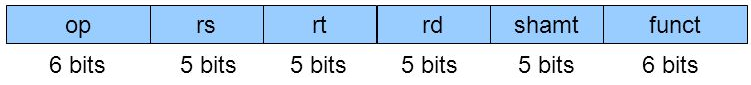
\includegraphics[width=0.5\linewidth]{slides/rtype}
		\end{center}
		\item I-type, istruzioni di tipo immediato, come LOAD, STORE, BRANCH, ADDi, SUBi
		\begin{center}
			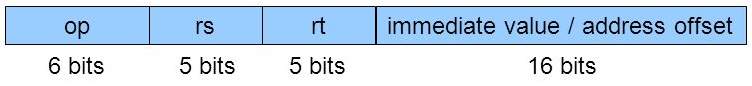
\includegraphics[width=0.5\linewidth]{slides/itype}
		\end{center}
		\item J-type, istruzioni di salto, come JUMP
		\begin{center}
			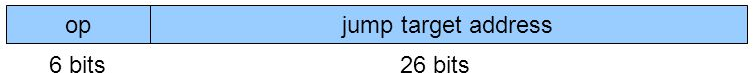
\includegraphics[width=0.5\linewidth]{slides/jtype}
		\end{center}
	\end{itemize}
	
		\subsection{ISA - Istruction Set Architecture}
		Queste CPU devono essere in grado di eseguire:
		Istruzioni R-type:
		\begin{itemize}[noitemsep]
			\item ADD
			\item SUB \\
			\item SLT  - Set on Less Then\\
			\item AND
			\item OR
		\end{itemize}
		Istruzioni I-type:
		\begin{itemize}[noitemsep]
			\item LW - Load Word
			\item SW - Store Word
			\item BEQ - Branch If Equal
			\item BNE - Branch if Not Equal
			\item ADDi - ADD Immediate
			\item SUBi - SUB Immediate
		\end{itemize}
		Istruzioni J-type:
		\begin{itemize}[noitemsep]
			\item J - Jump
		\end{itemize}
	
	\subsection{Scrivere sintassi e semantica delle operazioni MIPS BNE e SLT}
	L’istruzione BNE, branch if not equal, è di tipo immediate, ovvero I-Type. I primi 6 bit sono del campo operation, poi 5 bit del campo rs, altri 5 bit del campo rt e successivamente 26 bit per la costante immediata. Questa istruzione confronta i due registri rs e rt e se sono diversi salta all’istruzione indicata dal campo immediato (che è PC-relative). \\[2mm]
	L’istruzione SLT invece, set on less then, è di tipo R-Type. I primi 6 bit sono sempre dedicati al campo operation, i prossimi 15 bit sono quelli di 3 registri (da 5 bit ciascuno – rs,rt,rd) poi vi sono altri 5 bit che sono del campo shmat (shift amount, diversi da zero sono in caso di shifting) e gli ultimi 6 bit sono del campo funct (che determina il tipo dell’operazione). Questa istruzione confronta i due registri rt e rd e se rt < rd imposta rs a 1, altrimenti a 0.
	
	\subsection{Scrivere la semantica dell’istruzione assembler BEQ. Se all’indirizzo di memoria 2000FC00 è presente l’istruzione beq $5,$6,00A0 (indirizzo e costante espressi in esadecimale), quale sarebbe l’indirizzo target nel caso in cui il branch fosse taken?}
	
	L’istruzione BEQ, branch if equal, è di tipo immediate, ovvero I-Type. I primi 6 bit sono del campo operation, poi 5 bit del campo rs, altri 5 bit del campo rt e successivamente 26 bit per la costante immediata. Questa istruzione confronta i due registri rs e rt e se i contenuti sono uguali salta all’istruzione indicata dal campo immediato (che è PC-relative). Quindi se l’istruzione si trova all’indirizzo 2000FC00, ed è taken, l’indirizzo di salto sarà 2000FC00 + 00A0 = 2000FCA0.
	
	\subsection{Scrivere sintassi, semantica e formato delle seguenti istruzioni assembler: j, subi}
	L’istruzione Jump, salto incondizionato, aggiorna il PC con un nuovo indirizzo. L’istruzione j è, appunto, di tipo J-type, ed è formata da: 6 bit del campo operation e 26 bit per l’indirizzo (PC-relative). Per ottenere l’indirizzo di Jump devo: shiftare di 2 a sinistra l’indirizzo a 26 bit, e concatenare i primi 4 bit del PC a questi 28 bit appena ottenuti. Ottengo cosi un indirizzo a 32 bit da salvare nel PC. \\[2mm]
	L’istruzione SUBi, SUB immediate, è di tipo I-type. È formata da:
	\begin{itemize}[noitemsep]
		\item 6 bit di operation
		\item 5 bit del registro sorgente (rs)
		\item 5 bit del registro destinazione (rt)
		\item 16 bit per la costante immediata, che rappresenta il secondo operando
	\end{itemize}	
	La costante viene estesa a 32 bit quindi sommata ai 32 bit del contenuto del registro rs definito dai 5 bit di ingresso al Register File.
	
	\newpage
	
	\section{CPU Singolo Ciclo}
	\subsection{Principi di progetto, svantaggi e vantaggi}
	La CPU singolo ciclo deve essere in grado di eseguire una le seguenti istruzioni: lw, sw, add, sub, slt, and, or, beq, jump in un solo ciclo di clock. Quindi ogni istruzione (che è composta da più sub-attività) deve essere eseguita in un unico ciclo. Il clock va dimensionato in corrispondenza dell’istruzione che richiede più tempo di elaborazione. Questo però comporta che le istruzioni più corte, che impiegano meno tempo del periodo del clock vengano penalizzate (essendo il clock a tempo fisso).  Se ad esempio l’istruzione lw (load) richiede 5 sub-attività che impiegano 8 ms in totale e tutte le altre operazioni impiegano un tempo minore, il clock andrà dimensionato a minimo 8 ms, penalizzando, ad esempio, l’istruzione j (jump) che impiega solo 3 subs e 4 ms. I restanti 4 ms vengono sprecati dovendo la CPU attendere il nuovo ciclo di clock per iniziare l’istruzione successiva. Inoltre dovendo svolgere in un’unica istruzione più attività dello stesso genere (es. due somme, una per l’indirizzo di memoria e uno per incrementare il PC) nello stesso ciclo, siamo costretti a replicare le risorse che svolgono in questo caso la somma, in quanto la risorsa è già impegnata nella prima operazione quando è il momento di calcolare anche la seconda. Lo svantaggio principale di questa CPU è che (nel caso reale) dovendo svolgere operazioni FP, che richiedono molto tempo di elaborazione, il ciclo di clock venga allungato a dismisura, rallentando drasticamente i tempi di risposta.
	
	\section{CPU Multiciclo}
	
	\subsection{Tabella istruzioni/cicli}
	\begin{center}
		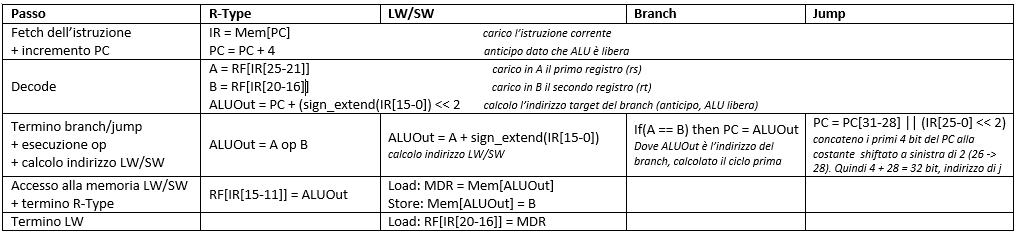
\includegraphics[width=1\linewidth]{slides/cpu.png}
	\end{center}	
	
	\subsection{Principi di progetto, svantaggi e vantaggi}
	La CPU multiciclo deve essere in grado di eseguire le stesse operazioni di quella a singolo ciclo, ma in un modo ottimizzato. Questa CPU non dovrà più eseguire un operazione intera nello stesso ciclo di clock, ma piuttosto dovrà ad ogni ciclo terminare una delle sotto attività richieste dall’istruzione principale. Per ottenere questo risultato dobbiamo introdurre nuovi registri e nuovi controlli, che tengano traccia del punto di esecuzione, ovvero che riescano a capire e tenere memorizzato che passi (subs) abbiamo già svolto. In questo caso non abbiamo più bisogno di un ciclo di clock lungo come l’istruzione che impiega più tempo, ma ci basterà un ciclo di clock che basti a terminare la sotto operazione più costosa in termini di tempo. Oltre al clock ridotto, inoltre, non abbiamo nemmeno più il problema della replicazione esagerata delle risorse, infatti nel caso di prima, ovvero quando nella stessa istruzione vi sono due operazioni simili (due somme), nel primo ciclo completo la prima somma, e nel ciclo successivo la seconda, evitando così di replicare risorse.
	
	\newpage
	\subsection{Passi di esecuzione delle istruzioni nella CPU multiciclo}
	\textbf{LOAD - 5 cicli}
	\begin{enumerate}[noitemsep, label=\arabic*)]
		\item Carico nel IR il contenuto della memoria indicato da PC e aggiorno il contatore di PC (PC = PC + 4)
		\item Carico nell’elemento di memoria A il contenuto del primo registro (rs) [e in B il contenuto del secondo. Nello stesso ciclo calcolo l’indirizzo del branch]
		\item Calcolo l’indirizzo da cui leggere i dati per scriverli nel registro. Quindi A + offset
		\item Carico nel MemoryDataRegister il contenuto della memoria indicato dall’indirizzo calcolato al ciclo precedente
		\item Carico nel registro rt il contenuto di MDR
	\end{enumerate}
	\textbf{STORE - 4 cicli}
	\begin{enumerate}[noitemsep, label=\arabic*)]
		\item Carico nel IR il contenuto della memoria indicato da PC e aggiorno il contatore di PC (PC = PC + 4)
		\item Carico nell’elemento di memoria A il contenuto del primo registro [e in B il contenuto del secondo. Nello stesso ciclo calcolo l’indirizzo del branch]
		\item Calcolo l’indirizzo in cui scrivere i dati letti dal registro il cui contenuto è in B
		\item Scrivo nella memoria (all'indirizzo calcolato al ciclo precedente) il contenuto di B
	\end{enumerate}	
	\textbf{BEQ, BNE - 3 cicli}
	\begin{enumerate}[noitemsep, label=\arabic*)]
		\item Carico nel IR il contenuto della memoria indicato da PC e aggiorno il contatore di PC (PC = PC + 4)
		\item Carico nell’elemento di memoria A il contenuto del primo registro e in B il contenuto del secondo
		\item Se il caso è taken (A==B / A!=B) imposto il valore di PC all’indirizzo calcolato dall’ALU nel ciclo precedente
	\end{enumerate}
	\textbf{	ADD, SUB - 4 cicli}
	\begin{enumerate}[noitemsep, label=\arabic*)]
		\item Carico nel IR il contenuto della memoria indicato da PC e aggiorno il contatore di PC (PC = PC + 4)
		\item Carico nell’elemento di memoria A il contenuto del primo registro e in B il contenuto del secondo. [Nello stesso ciclo calcolo l’indirizzo del branch]
		\item Calcolo il risultato l’operazione (ADD/SUB) tra il contenuto di A e B
		\item Scrivo nel registro destinazione (rd) il risultato proveniente dall'ALU dal ciclo precedente
	\end{enumerate}
	\subsection{La CPU multiciclo vista a lezione utilizza per l’esecuzione delle istruzioni SUB e LW rispettivamente 4 e 5 cicli di clock. Descrivere brevemente cosa accade nei vari cicli per le due istruzioni}
	L’operazione SUB, sottrazione, è di tipo aritmetico-logico, quindi R-type. Al primo ciclo carico nel Istruction Register il contenuto della memoria indicato dal PC e nello stesso ciclo incremento il valore di PC (PC = PC + 4). Nel ciclo successivo carico nell’elemento di memoria A il contenuto del Register File indicato dall'Istruction Register in base ai 5 bit del primo suo ingresso (rs) e svolgo lo stesso compito anche per l’elemento di memoria B (scrivo in B rt). In questo stesso ciclo calcolo l’indirizzo del branch nel caso fosse taken (passo di anticipo). A questo punto ho i due addenti dell’operazione negli elementi A e B, e faccio eseguire all’ALU l’operazione richiesta (SUB). A questo punto scrivo nel registro identificato da rd il risultato dell’ALU.\\[2mm]
	L'istruzione LW, Load Word, carica in un registro il contenuto di una cella di memoria. E' di tipo I-type ed impiega 5 cicli di esecuzione. Al primo ciclo (1) carico l'istruzione corrente, indicata dal PC. AL ciclo successivo (2) carico nell'elemento di memoria A il contenuto del rispettivo registro (rs). Nel ciclo successivo (3) calcolo l'indirizzo dal quale prendere i dati (determinato dalla somma di A + il campo immediate, che è l'offset). Al ciclo successivo (4) carico nel Memory Data Register il contenuto della cella di memoria calcolata al ciclo precedente. All'ultimo ciclo (5) carico nel registro (rt) il contenuto dell'MDR, caricato precedentemente con il contenuto della cella di memoria desiderata.
	
	\newpage
	\section{Hardware}
	\subsection{Register File}
	Il Register File, contenuto nel datapath e formato da 32 registri (ognuno dei quali è a 32 bit, formati a loro volta da 32 flip-flop) è un elemento di memoria che contiene, ad esempio, gli addendi di un’operazione aritmetico-logica. Deve permettere la lettura di 2 registri e la scrittura di 1 registro. Il clock viene messo in AND con un segnale di controllo Write e trasmesso a tutti i registri. Il segnale determina se in corrispondenza della discesa del clock il valore in input debba essere memorizzato o meno. È composto da 
	\begin{itemize}[noitemsep]
		\item 3 ingressi a 5 bit che rappresentano i due registri da leggere (rs,rt) e quello da scrivere (rd)
		\item Un ingresso a 32 bit che rappresenta il dato da andare a scrivere nel registro
		\item 2 uscite a 32 bit che rappresentano il contenuto dei registri letti
	\end{itemize}	
	Il Register file fornisce sempre in output una coppia di registri, non significativi, se i controlli di lettura non lo sono, in tal caso, i circuiti che potenzialmente potrebbero usarli, devono ignorali.
	
	\subsection{Descrivere come avvengono le operazioni di lettura e scrittura nel Register File}
	Nel register file tutti i registri (32) sono collegati a due multiplexer 32:1 che ricevono come segnale di controllo i due ingressi a 5 bit che rappresentano i due registri dei quali si vuole ottenere il contenuto. A questo punto i 5 bit del primo registro vengono usati come input del primo MUX e i 5 bit del secondo registro come input del secondo MUX. Il register file fornisce sempre in output una coppia di registri, ma che non sono significativi se i controlli a 5 bit del MUX non lo sono. In questo caso i circuiti che potenzialmente potrebbero usarli devono ignorarli. \\[2mm]
	Per la scrittura invece tutti i registri sono in AND con un segnale di Write (a sua volta in AND con il clock) e con l’uscita di un decoder che decodifica il segnale di controllo in ingresso a 5 bit WriteReg\#. Nel caso il clock o il Write non siano affermati, i possibili valori spuri non vengono memorizzati.
	
	\subsection{SRAM - Static RAM}
	La SRAM è più veloce della memoria principale, infatti per la sua realizzazione vengono utilizzati dei latch. E' utilizzata per le memorie veloci, come le cache (tempi di accesso $0.5 - 2.5$ ns). \\[2mm]
	E' realizzata come matrice di latch $H\times W$ dove
	\begin{itemize}[noitemsep]
		\item W è l'ampiezza, ovvero il numero di latch per ogni cella
		\item H è l'altezza, ovvero il numero di celle indirizzabili
	\end{itemize}
	Per ragioni costruttive W è spesso piccolo, e non è possibile leggere e scrivere contemporaneamente.\\\\
	Esempio di chip $32K\times8$, 32K celle da 8 bit = 256Kb
	\begin{center}
		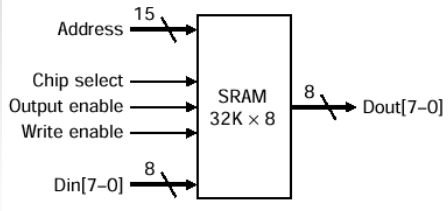
\includegraphics[width=0.3\linewidth]{slides/sram}
	\end{center}

	
	\newpage
	\section{Circuiti sequenziali}
	\subsection{S-R Latch}
	L’S-R Latch è un circuito, composto da due porte NOR concatenate, che costituisce elemento base per costruire elementi di memoria più complessi come i flip-flop. S equivale a SET, mentre R equivale a RESET. L’input del circuito sono dunque 2 bit, S e R:
	\begin{itemize}[noitemsep]
		\item S=0, R=0: combinazione di riposo, il bit memorizzato non viene modificato
		\item S=1,R=0: combinazione di set, viene memorizzato il valore 1
		\item S=0,R=1: combinazione di reset, viene memorizzato il valore 0
		\item S=1,R=1: combinazione che non deve mai essere presentata al circuito, in quanto accadrebbe che Q = $\lnot$Q = 0
	\end{itemize}
	\begin{center}
		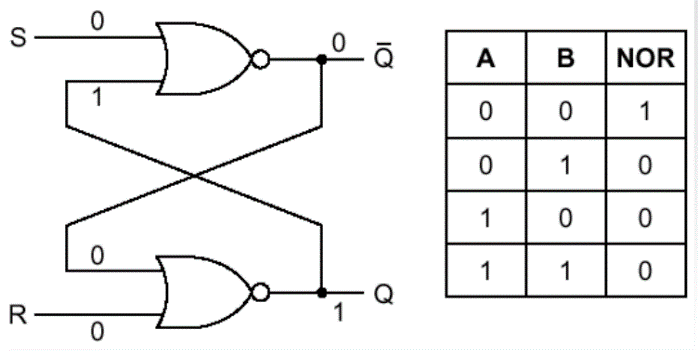
\includegraphics[width=0.4\linewidth]{slides/latch.png}
	\end{center}
	
	\subsection{Latch clockato (D-latch)}
	Ha lo stesso funzionamento del S-R Latch, solo che con l'aggiunta delle porte AND a monte non può mai verificarsi la condizione S=R=1 in input. \\[2mm]
	Nota che durante il periodo alto del clock il latch non esercita alcuna azione di memorizzazione. Il valore D non è stabilizzato durante il livello alto del clock, infatti può variare più volte fino alla stabilizzazione (periodo basso). Questo fenomeno è detto trasparenza del Latch.
	\begin{center}
		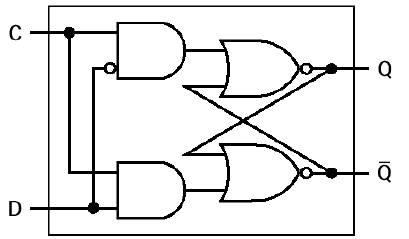
\includegraphics[width=0.3\linewidth]{slides/dlatch.png}
	\end{center}	

	\subsection{Flip-flop semplice}
	E' un elemento di memoria che memorizza pressoché istantaneamente un valore D fornitogli in ingresso in corrispondenza del fronte di salita del clock (dell’impulso generato dalla salita). È un elemento edge-triggered di tipo rising triggered. Il generatore di impulsi che utilizza il flip-flop sfrutta il ritardo di propagazione delle porte per generare un impulso brevissimo in corrispondenza del fronte di salita del clock.
	\begin{center}
		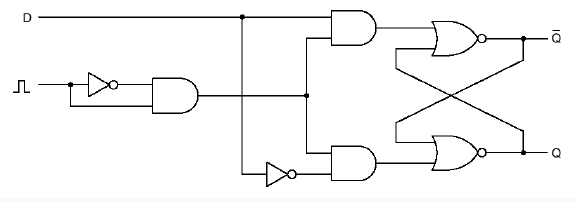
\includegraphics[width=0.6\linewidth]{slides/flip-flop.png}
	\end{center}
	
	\section{Prestazioni di un sistema}
	\subsection{Formule per la misurazione delle prestazioni}
	\begin{itemize}
		\item Il tempo di esecuzione di un programma è definito come
			\[
				\begin{split}
					\text{T}_{\text{exe}} &= \text{\# cicli} \cdot T \\[2mm] &= \dfrac{\text{\# cicli} }{F}  \\[2mm] &= IC \cdot CPI \cdot T \\[2mm] &= \dfrac{IC \cdot CPI}{F}
				\end{split}
			\]		
		\item Performance:
			\[
				\text{perf}_A = \dfrac{1}{\text{T}_{\text{exe}}}
			\]
		\item Il numero di cicli:
			\[
				\text{\# cicli} = IC \cdot CPI
			\]
		\item MIPS, milioni di istruzioni per secondo:
			\[
				\begin{split}
					\text{MIPS} &= \dfrac{IC}{\text{T}_{\text{exe}} \cdot 10^6} \\[2mm] &= \dfrac{IC}{IC \cdot \frac{CPI}{F} \cdot 10^6} \\[2mm] &= \dfrac{F}{CPI \cdot 10^6}
				\end{split}
			\]
		\item SpeedUp, indica quante volte la macchina $A$ è più veloce della macchina $B$:
		\[
			\begin{split}
				\text{speedUp} &= \dfrac{\text{T}_{\text{exe}A}}{\text{T}_{\text{exe}B}} \\[2mm]
				&= \dfrac{\text{perf}_A}{\text{perf}_B}
			\end{split}
		\] 
	\end{itemize}
	\subsection{Cos'è, e a cosa serve la Legge di Amdahl? Scrivere la formula e descrivere il significato delle varie componenti}
	
	
	La legge di Amdahl fissa un limite agli incrementi di prestazioni ottenibili (Speedup) quando introduciamo delle ottimizzazioni.\\[2mm]
	La legge di Amdahl è definita come
		\[
			T_{\text{ott}} = \dfrac{1}{s}\cdot T_{\text{exe}} + \dfrac{\left(1 - \frac{1}{s} \right) \cdot 	T_{\text{exe}}}{n}
		\]
	dove 
	\begin{itemize}
		\item $\frac{1}{s} \cdot \text{T}_{\text{exe}}$ è la frazione del tempo di esecuzione \underline{non} modificata dalle ottimizzazioni
		\item $\left( 1 - \frac{1}{s} \right) \cdot \text{T}_{\text{exe}}$ è la frazione del tempo di esecuzione modificata dalle ottimizzazioni
		\item $n$ è il fattore del miglioramento ottenuto tramite le ottimizzazioni
	\end{itemize}
\end{document}